\documentclass[a4paper,12pt]{extarticle}
\usepackage[utf8x]{inputenc}
\usepackage[T1,T2A]{fontenc}
\usepackage[russian]{babel}
\usepackage{hyperref}
\usepackage{indentfirst}
\usepackage{listings}
\usepackage{color}
\usepackage{here}
\usepackage{array}
\usepackage{multirow}
\usepackage{graphicx}
\usepackage{algorithm}
\usepackage{algpseudocode}
\usepackage{caption}
\usepackage{pdfpages}
\usepackage{tikz,mathpazo}
\usepackage{graphicx,amssymb,amstext,amsmath,newtxmath}
\usetikzlibrary{shapes.geometric, arrows}
\renewcommand{\lstlistingname}{Программа} % заголовок листингов кода

\bibliographystyle{ugost2008ls}

\usepackage{listings}
\lstset{ %
extendedchars=\true,
keepspaces=true,
language=C,						% choose the language of the code
basicstyle=\footnotesize,		% the size of the fonts that are used for the code
numbers=left,					% where to put the line-numbers
numberstyle=\footnotesize,		% the size of the fonts that are used for the line-numbers
stepnumber=1,					% the step between two line-numbers. If it is 1 each line will be numbered
numbersep=5pt,					% how far the line-numbers are from the code
backgroundcolor=\color{white},	% choose the background color. You must add \usepackage{color}
showspaces=false				% show spaces adding particular underscores
showstringspaces=false,			% underline spaces within strings
showtabs=false,					% show tabs within strings adding particular underscores
frame=single,           		% adds a frame around the code
tabsize=2,						% sets default tabsize to 2 spaces
captionpos=t,					% sets the caption-position to top
breaklines=true,				% sets automatic line breaking
breakatwhitespace=false,		% sets if automatic breaks should only happen at whitespace
escapeinside={\%*}{*)},			% if you want to add a comment within your code
postbreak=\raisebox{0ex}[0ex][0ex]{\ensuremath{\color{red}\hookrightarrow\space}},
texcl=true,
inputpath=listings,                     % директория с листингами
}

\usepackage[left=2cm,right=2cm,
top=2cm,bottom=2cm,bindingoffset=0cm]{geometry}

%% Нумерация картинок по секциям
\usepackage{chngcntr}
\counterwithin{figure}{section}
\counterwithin{table}{section}

%%Точки нумерации заголовков
\usepackage{titlesec}
\titlelabel{\thetitle.\quad}
\usepackage[dotinlabels]{titletoc}

%% Оформления подписи рисунка
\addto\captionsrussian{\renewcommand{\figurename}{Рисунок}}
\captionsetup[figure]{labelsep = period}

%% Подпись таблицы
\DeclareCaptionFormat{hfillstart}{\hfill#1#2#3\par}
\captionsetup[table]{format=hfillstart,labelsep=newline,justification=centering,skip=-10pt,textfont=bf}

%% Путь к каталогу с рисунками
\graphicspath{{fig/}}

%% Внесение titlepage в учёт счётчика страниц
\makeatletter
\renewenvironment{titlepage} {
 \thispagestyle{empty}
}
\makeatother


\begin{document}	% начало документа

% Титульная страница
\begin{titlepage}	% начало титульной страницы

	\begin{center}		% выравнивание по центру

		\large Санкт-Петербургский политехнический университет Петра Великого\\
		\large Физико-механический институт \\
		\large Высшая школа прикладной математики и вычислительной физики\\[3cm]
		% название института, затем отступ 6см
		\large Направление подготовки\\
		\large "01.03.02. Прикладная математика и информатика"\\[3cm]
		\huge Дисциплина "Численные методы"\\[0.5cm] % название работы, затем отступ 0,5см
		\large Отчет по лабораторной работе №3\\[0.1cm]
		\large "Решение СЛАУ итерационными методами. Метод простых итераций"\\[5cm]

	\end{center}


	\begin{flushright} % выравнивание по правому краю
		\begin{minipage}{0.25\textwidth} % врезка в половину ширины текста
			\begin{flushleft} % выровнять её содержимое по левому краю

				\large\textbf{Работу выполнил:}\\
				\large Иванова А.С.\\
				\large {Группа:} 5030102/00002\\
				
				\large \textbf{Преподаватель:}\\
				\large Курц В.В.

			\end{flushleft}
		\end{minipage}
	\end{flushright}
	
	\vfill % заполнить всё доступное ниже пространство

	\begin{center}
	\large Санкт-Петербург\\
	\large \the\year % вывести дату
	\end{center} % закончить выравнивание по центру

\end{titlepage} % конец титульной страницы

\vfill % заполнить всё доступное ниже пространство


% Содержание
\renewcommand\contentsname{\centerline{Содержание}}
\tableofcontents
\newpage



\section{Формулировка задачи}

Необходимо решить краевую задачу для дифференциального уранвения 2-го порядка методом конечных разностей.

\begin{equation}
	\begin{cases}
		p(x)y''+q(x)y'+r(x)y=f(x) \\
		y(a)= A \\
		y(b) = B 	
	\end{cases}
\end{equation}

Исходная функция: 
\begin{equation}
	(2x+1)xy''+(2x+2)y'-y=\frac{1}{x} \\
\end{equation}

На отрезке [0.2;1] с граничными условиями

\begin{math}
	y(0.2)= 5 ;
	y(1) = 1 
\end{math}

Известно точное решение:

\begin{math}
	y=\frac{1}{x}
\end{math}

Необходимо исследовать сходимость метода, влияние шага на точность вычислений, влияние ошибок в исходных данных на решение, т.е. устойчивость задачи и ошибку в вычислениях при заданном шаге на разных участках равномерной сетки. 

\section{Алгоритм метода и условия его применимости}


\subsection{Алгоритм метода}

Рассмотрим краевую задачу: 

\begin{equation}
	\begin{cases}
		p(x)y''+q(x)y'+r(x)y=f(x), x \in [a,b] \\
		y(a)= A \\
		y(b) = B 	
	\end{cases}
\end{equation}

Построим равномерную сетку на [a, b]:

N - Количество разбиений равномерной сетки

\begin{math}
	h = \frac{b-a}{N}; x_{i}=a+h*i; i=0,...,N
\end{math}

Запишем ОДУ в узлах сетки: 

\begin{math}
	p_{k}y''+q_{k}y'+r_{k}y=f_{k}, k=0,...,N
\end{math}

где 

\begin{math}
	p_{k}=p(x_{k}), q_{k}=q(x_{k}), r_{k}=r(x_{k}), f_{k}=f(x_{k})
\end{math}

Далее аппроксимируем производные конечно-разностными выражениями и получаем: 

 
\begin{math}
	y''(x)=\frac{y(x+h)-2y(x)+y(x-h)}{h^{2}}+O(h^{2})
\end{math}

\begin{math}
	y'(x)=\frac{y(x+h)+y(x-h)}{2h}+O(h^{2})
\end{math}

Заменим в этих выражениях \begin{math}
	x
\end{math} на 
\begin{math}
	x_{k}
\end{math} , подставим в исходное дифференциальное уравнение, заменим \begin{math}
y(x_{k})
\end{math} на \begin{math}
y_{k}
\end{math} и отбросим 
\begin{math}
	O(h^{2})
\end{math}

Получаем: 

\begin{equation}
	p_{k}\frac{y_{k+1}-2y_{k}+y_{k-1}}{h^{2}}+q_{k}\frac{y_{k+1}-y_{k-1}}{2h}+r_{k}y_{k}=f_{k}, k=1,...,N-1 \\
\end{equation}

Вынесем за скобки \begin{math}
	y_{k}
\end{math} и с учетом граничных условий получим систему уравнений:

\begin{equation}
	\begin{cases}
		(p_{k}-\frac{q_{k}}{2}h)y_{k-1}+(h^{2}r_{k}-2p_{k})y_{k}+(p_{k}+\frac{q_{k}}{2}h)y_{k+1}=h^{2}f_{k}, k=1,...,N-1 \\
		y_{0}= A \\
		y_{N} = B 	
	\end{cases}
\end{equation}

С учетом граничных условий данная система уравнений образует трехдиагональную матрицу. Такая система решается методом прогонки для трехдиагональных матриц.

\subsection{Условия применимости}

\begin{itemize}
	\item Частная производная по х непрерывна и ограничена
	\item Выполянется условие Липшица по y
	\begin{equation}
		|f(x,y_{1})-f(x,y_{2})| \leq L|y_{1}-y_{2}|
	\end{equation}
	\item Существование непрерывных производных до 2-го порядка для применения правила Рунге.
	\item Теорема: 
	
	Если  \begin{math}
	 \forall	x \in [a,b]
	\end{math} выполняется:

\begin{equation}
	\begin{cases}
		p(x) \geq 0 \\
		p(x) \geq \frac{h}{2}|q(x)| \\
		r(x) \leq 0
	\end{cases}
\end{equation}
 
 то СЛАУ имеет единственное решние и вычислительная погрешность \begin{math}
 	O(h^{2})
 \end{math}

\end{itemize}


\section{Предварительный анализ задачи}

Для оценки погрешности используется правило Рунге:

\begin{equation} 
	\frac{|S_{n,2N}(f)-S_{n,N}(f)|}{2^{m}-1} \leq \epsilon
\end{equation}

Для МКР m=2

\section{Проверка условий применимости метода}

Исходная функция: 
\begin{equation}
	(2x+1)xy''+(2x+2)y'-y=\frac{1}{x} \\
\end{equation}

На отрезке [0.2;1]

Данная функция будет иметь разрывы производных по х в точках 0 и -0.5, которые не входят в заданный отрезок. Условие Липшица по у выполнено. 

В данном случае: 

\begin{math}
	p(x) = (2x+1)x ; 	q(x) = 2x+2 ;	r(x) = -1 
\end{math}

Очевидно, что условия теоремы выполняются и СЛАУ, которую необходимо решить будет иметь единственное решение. 

\section{Тестовый пример с детальными расчетами для задачи малой размерности}

Решим краевую задачу для дифференциального уранвения 2-го порядка: 

\begin{equation}
	(2x+1)xy''+(2x+2)y'-y=\frac{1}{x} \\
\end{equation}

На отрезке [0.2;1] с граничными условиями

\begin{math}
	y(0.2)= 5 ;
	y(1) = 1 
\end{math}

В данном случае: 

\begin{math}
	p(x) = (2x+1)x ; 	q(x) = 2x+2 ;	r(x) = -1 ; f(x)=\frac{1}{x}
\end{math}

Пусть N=2, тогда h=0.6

Получаем линейное уравнение: 

\begin{equation}
  (p_{1}-\frac{q_{1}}{2}h)y_{0}+(h^{2}r_{1}-2p_{1})y_{1}+(p_{1}+\frac{q_{1}}{2}h)y_{2}=h^{2}f_{1}
\end{equation}

\begin{equation}
	(1.32-\frac{3.2}{2}*0.4)*5+(0.4^{2}*(-1)-2*1.32)y_{1}+(1.32+\frac{3.2}{2}*0.4)*1=0.4^{2}*\frac{5}{3}
\end{equation}
  
Получаем 

\begin{math}
	y_{1}=2
\end{math}

Пусть N=4, тогда h=0.2 

Равномерная сетка: \begin{math}
	\{0.2;0.4;0.6;0.8;1\}
\end{math}

Получаем систему из трех уравнений: 

\begin{equation}
	\begin{cases}
		(p_{1}-\frac{q_{1}}{2}h)y_{0}+(h^{2}r_{1}-2p_{1})y_{1}+(p_{1}+\frac{q_{1}}{2}h)y_{2}=h^{2}f_{1} \\
		(p_{2}-\frac{q_{2}}{2}h)y_{1}+(h^{2}r_{2}-2p_{2})y_{2}+(p_{2}+\frac{q_{2}}{2}h)y_{3}=h^{2}f_{2} \\
		(p_{3}-\frac{q_{3}}{2}h)y_{2}+(h^{2}r_{3}-2p_{3})y_{3}+(p_{3}+\frac{q_{3}}{2}h)y_{2}=h^{2}f_{3} \\	
	\end{cases}
\end{equation}

\begin{equation}
	\begin{cases}
		(0.72-\frac{2.8}{2}*0.2)*5+(0.2^{2}*(-1)-2*0.72)y_{1}+(0.72+\frac{2.8}{2}*0.2)*y_{2}=0.2^{2}*2.5 \\
		(1.32-\frac{3.2}{2}*0.4)*y_{1}+(0.2^{2}*(-1)-2*1.32)y_{2}+(1.32+\frac{3.2}{2}*0.4)*y_{3}=0.2^{2}*\frac{5}{3} \\
		(2.08-\frac{3.6}{2}*0.2)*y_{2}+(0.2^{2}*(-1)-2*2.08)y_{3}+(2.08+\frac{3.6}{2}*0.4)*1=0.2^{2}*1.25 \\	
	\end{cases}
\end{equation}

\begin{equation}
	\begin{cases}
		 -1.48y_{1}+y_{2}=-2.1 \\
		 y_{1}-2.68y_{2}+1.64y_{3}=0.0667 \\
		 1.72y_{2}-4.2y_{3}=-2.39 \\	
	\end{cases}
\end{equation}

Решаем систему методом прогонки и получаем результат: 

Сеточная функция:
\begin{math}
	\{5, 2.5776, 1.7149, 1.2713, 1\}
\end{math}

Результат стал точнее, чем на предыдущей итерации

\section{Перечень контрольных тестов для иллюстрации метода}

  Необходимо решить краевую задачу методом конечных разностей:
 
\begin{equation}
	\begin{cases}
		p(x)y''+q(x)y'+r(x)y=f(x) \\
		y(a)= A \\
		y(b) = B 	
	\end{cases}
\end{equation}

 
 Исходная функция: 
\begin{equation}
	y''=\frac{-(2x+2)*y'*x+y*x+1}{x^{2}*(2x+1)}\\
\end{equation}
 На отрезке [0.2;1] с граничными условиями
 
 \begin{math}
 	y(0.2)= 5 ;
 	y(1) = 1 
 \end{math}
 
 
 Исследуется сходимость метода (количество итераций от заданной точности), влияние шага h на точность вычислений и влияние ошибок в исходных данных на решение, т.е. устойчивость задачи и ошибку в вычислениях при заданном шаге на разных участках равномерной сетки (берется h=0.0002 и вычисляется абсолютная ошибка вычислений во всех узлах сетки).

\section{Модульная структура программы}

def p(x):

def q(x):

def r(x):

def f(x):

Компоненты при y'', y', y и свободный член уравнения

def answer(x):

Точный результат

def FiniteDifferenceMethod(p, q, r, f, x0, y0, xn, yn, N):

Вычисление значения одной итерации метода конечных разностей при заданном количестве разбиений

def iterations(eps , p, q, r, f, x0, y0, xn, yn):

Получение решения краевой задачи методом конечных разностей с заданной точностью.

\section{Численный анализ решения задачи}

\subsection{Сходимость метода}

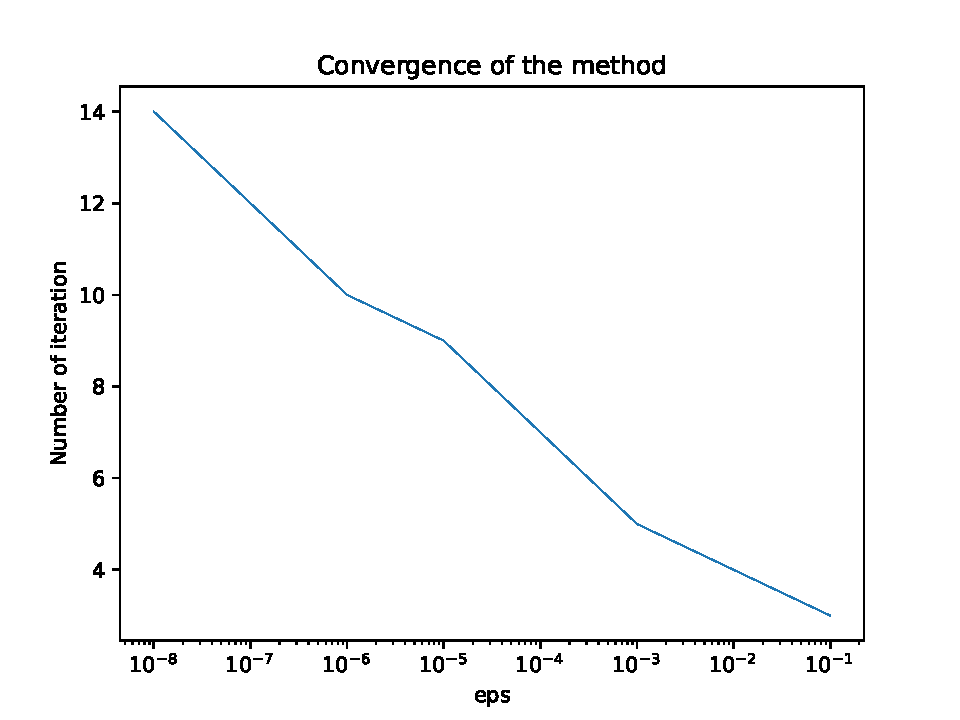
\includegraphics[scale=0.75]{1.pdf}

Из данного графика можно сделать вывод, что при увеличении количества итераций точность вычислений увеличивается

\subsection{Влияние шага на точность вычислений}

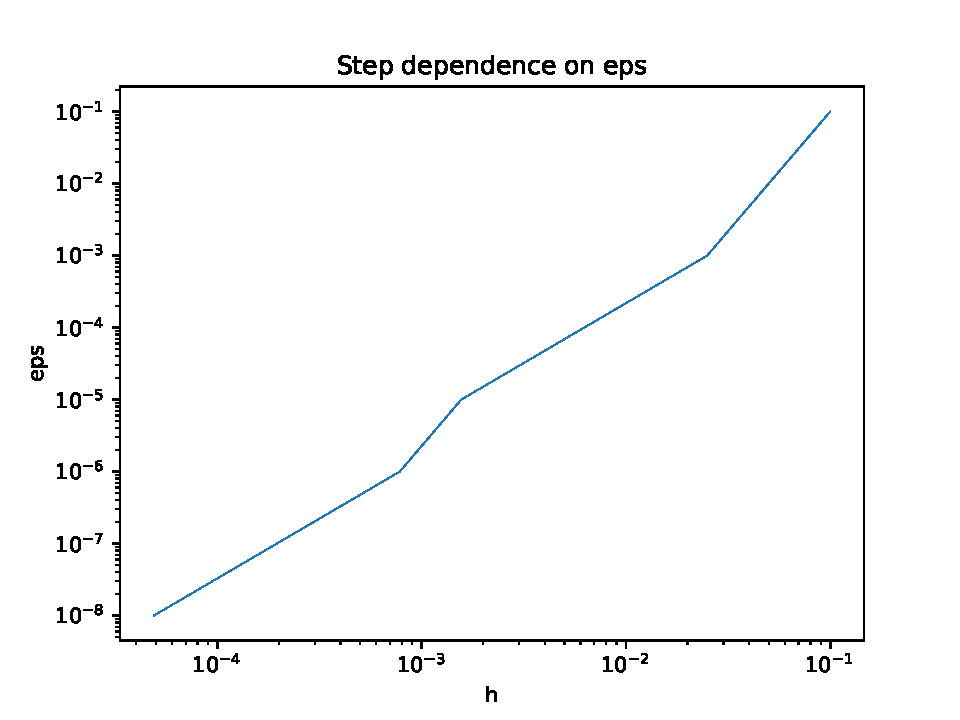
\includegraphics[scale=0.75]{2.pdf}

Из данного графика можно сделать вывод, что для достижения большей точности нужно уменьшать шаг равномерной сетки.

\subsection{Влияние ошибки исходных данных на решение}

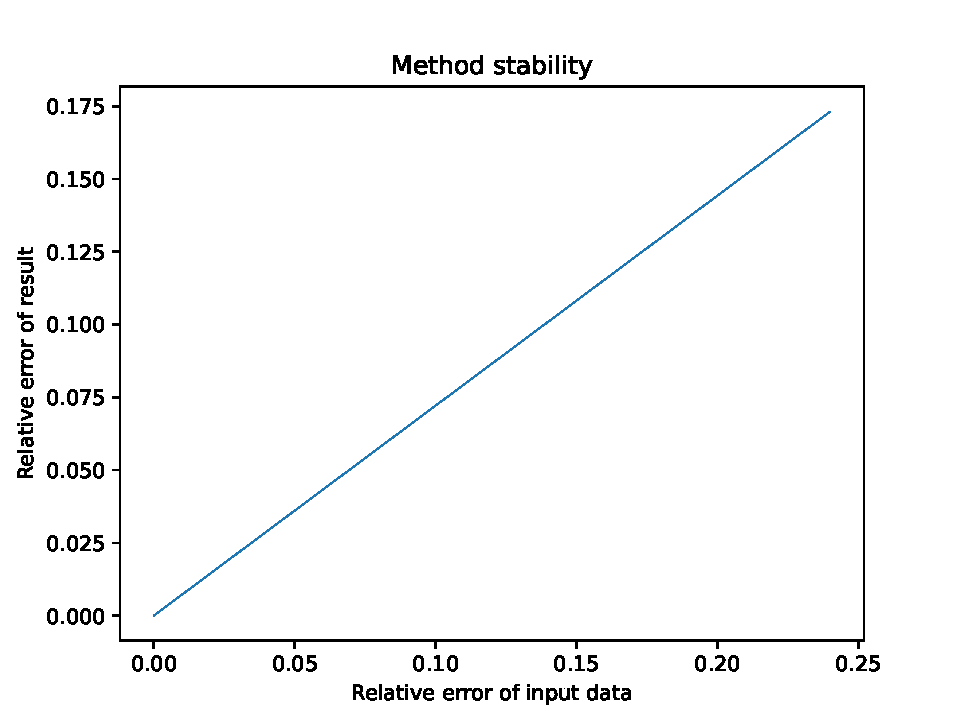
\includegraphics[scale=0.75]{3.pdf}

Из данного графика можно сделать вывод, что при увеличении ошибки в исходных данных ошибка вычислений увеличивается. Данная задача является устойчивой, т.к. ошибка входных данных и ошибка результата имеют одинаковый порядок.

\subsection{Ошибка вычислений на разных участках равномерной сетки}

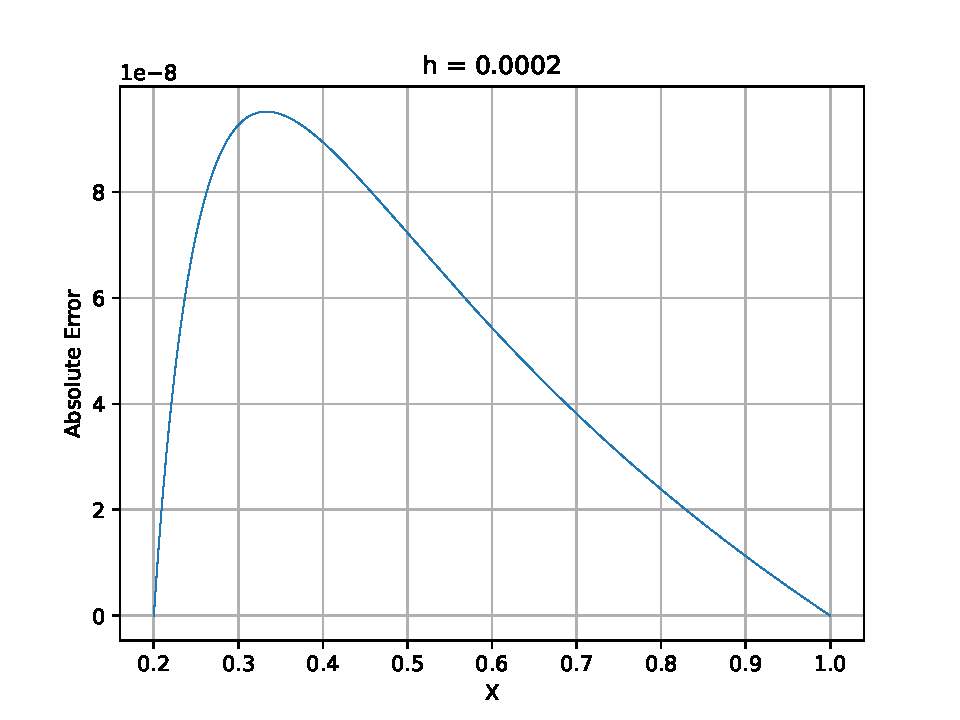
\includegraphics[scale=0.5]{4.pdf}
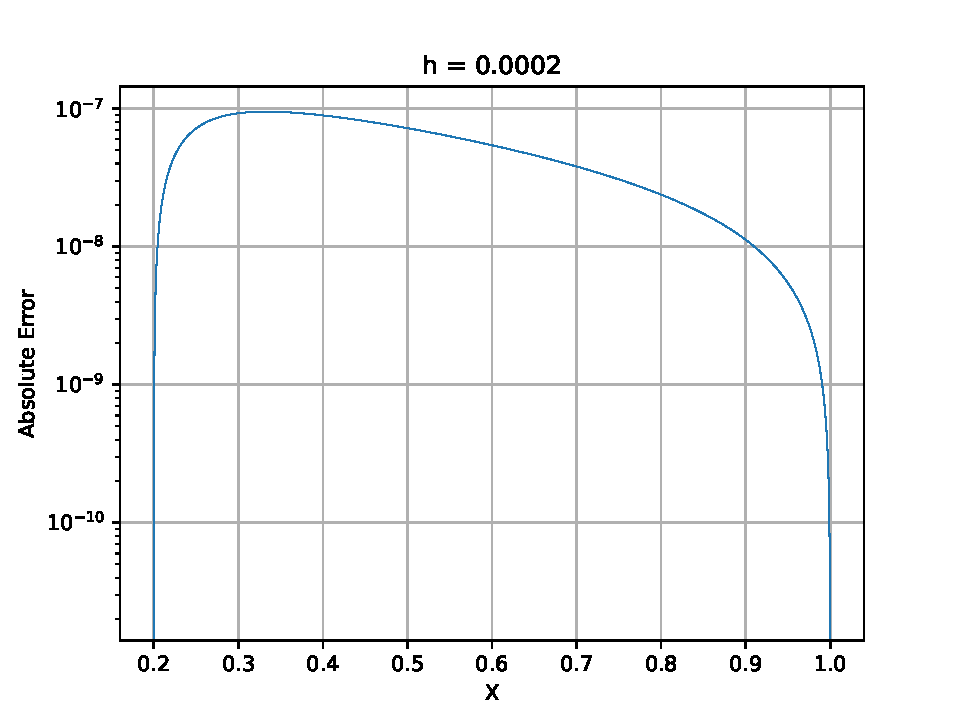
\includegraphics[scale=0.5]{5.pdf}


Из данного графика можно сделать вывод, что ошибка вычислений будет наименьшей ближе к краевым точкам отрезка, т.е к точкам 0.2 и 1. Для конкретно данной функции ошибка будет наибольшей на отрезке [0.3,0.4], далее будет постепенно убывать. 


\section{Краткие выводы}

На основе полученных результатов можно сделать вывод о том, что при увеличении количества итераций для метода конечных разностей и шага разбиения равномерной сетки погрешность результата уменьшается. Также можно сделать вывод о том, что если в исходные данные вносить ошибки, то при ее увеличении будет увеличиваться и ошибка результата. Данная задача является устойчивой, т.к. ошибка входных данных и ошибка результата имеют одинаковый порядок. Ошибка выичслений будет наименьшей на тех участках равномерной сетки, которые находятся ближе к кравеым узлам сетки. 

\end{document}
